\chapter{\IfLanguageName{dutch}{Stand van zaken}{State of the art}}%
\label{ch:stand-van-zaken}

In dit hoofdstuk van de bachelorproef zullen we dieper ingaan op het concept van een microservices-architectuur. Dit zal gebeuren aan de hand van een relevante literatuurstudie. Allereerst zal uitgelegd worden wat een monolithische architectuur is en wat typerend is aan deze stijl van software ontwikkeling. Daarna wordt uitgelegd wat een microservices-architectuur is en hoe deze architectuur verschilt van de klassieke, monolithische aanpak. Tot slot worden enkele relevante termen uitgebreider behandelt die de werking en structuur van microservices definiëren.

\section{Wat is een monolithische architectuur?}

De monolithische architectuur is door de jaren heen een succesvolle keuze geweest voor softwareontwikkelaars \autocite{Gos2020}. Bij deze aanpak van software ontwikkeling bestaat een applicatie uit verscheidene componenten. Voorbeelden van componenten zijn authenticatie en authorizatie, productbeheer, klantenbeheer enz. Deze componenten bevinden zich in een monolithische architectuur dan in één en hetzelfde programma.

\begin{figure}[H]
  \centering
  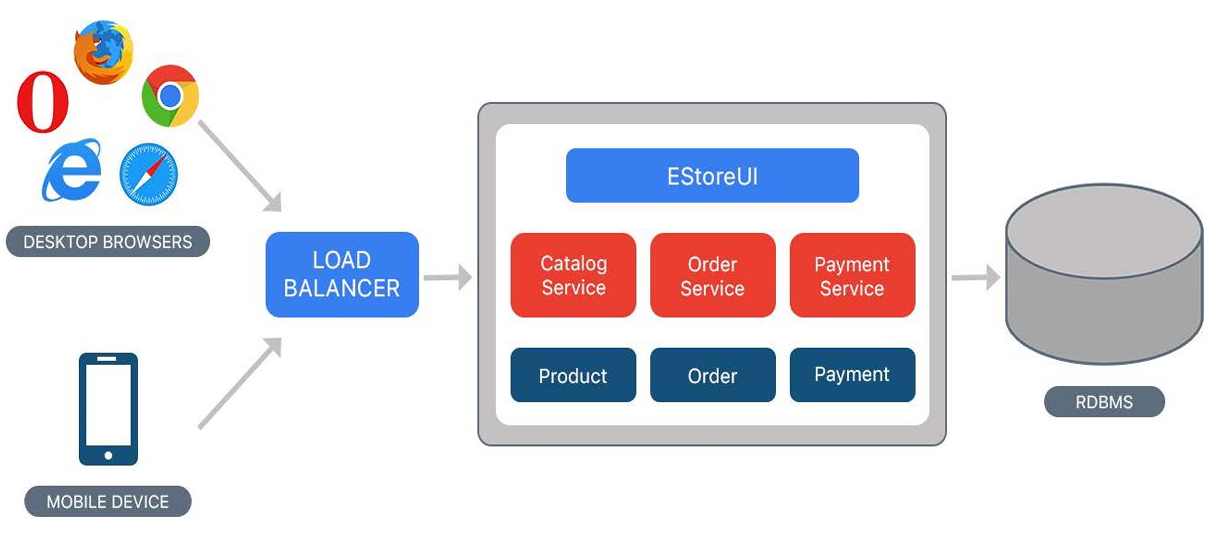
\includegraphics[width=0.8\textwidth]{MonolithischeArchitectuur.png}
  \caption[Voorstelling van een monolitische architectuur]{\label{fig:monolithische architectuur}Voorbeeld van een monolithische architectuur. Deze afbeelding toont de architectuur van een applicatie die de bedrijfslogica voor een e-commerce demonstreert \autocite{Gos2020}.}
\end{figure}

De bovenstaande afbeelding (Figuur \ref{fig:monolithische architectuur}) verduidelijkt de werking van een monolithische applicatie. In deze representatie zien we een EStoreUI component die fungeert als de grafische interface waarmee gebruiker kunnen interageren. Daaronder zijn 3 services gedefiniëerd, namelijk de Catalog Service, Order Service en Payment Service. Elk van deze 3 services is verantwoordelijk voor een specifiek bedrijfsproces. Vervolgens zijn alle services verbonden met eenzelfde relationele database (RDBMS). 

\section{Wat is een microservices-architectuur?}


% Tip: Begin elk hoofdstuk met een paragraaf inleiding die beschrijft hoe
% dit hoofdstuk past binnen het geheel van de bachelorproef. Geef in het
% bijzonder aan wat de link is met het vorige en volgende hoofdstuk.

% Pas na deze inleidende paragraaf komt de eerste sectiehoofding.

%Dit hoofdstuk bevat je literatuurstudie. De inhoud gaat verder op de inleiding, maar zal het onderwerp van de bachelorproef *diepgaand* uitspitten. De %bedoeling is dat de lezer na lezing van dit hoofdstuk helemaal op de hoogte is van de huidige stand van zaken (state-of-the-art) in het %onderzoeksdomein. Iemand die niet vertrouwd is met het onderwerp, weet nu voldoende om de rest van het verhaal te kunnen volgen, zonder dat die er nog %andere informatie moet over opzoeken \autocite{Pollefliet2011}.

%Je verwijst bij elke bewering die je doet, vakterm die je introduceert, enz.\ naar je bronnen. In \LaTeX{} kan dat met het commando %\texttt{$\backslash${textcite\{\}}} of \texttt{$\backslash${autocite\{\}}}. Als argument van het commando geef je de ``sleutel'' van een ``record'' in %een bibliografische databank in het Bib\LaTeX{}-formaat (een tekstbestand). Als je expliciet naar de auteur verwijst in de zin (narratieve %referentie), gebruik je \texttt{$\backslash${}textcite\{\}}. Soms is de auteursnaam niet expliciet een onderdeel van de zin, dan gebruik je %\texttt{$\backslash${}autocite\{\}} (referentie tussen haakjes). Dit gebruik je bv.~bij een citaat, of om in het bijschrift van een overgenomen %afbeelding, broncode, tabel, enz. te verwijzen naar de bron. In de volgende paragraaf een voorbeeld van elk.

%\textcite{Knuth1998} schreef een van de standaardwerken over sorteer- en zoekalgoritmen. Experten zijn het erover eens dat cloud computing een %interessante opportuniteit vormen, zowel voor gebruikers als voor dienstverleners op vlak van informatietechnologie~\autocite{Creeger2009}.

%Let er ook op: het \texttt{cite}-commando voor de punt, dus binnen de zin. Je verwijst meteen naar een bron in de eerste zin die erop gebaseerd is, %dus niet pas op het einde van een paragraaf.

%\begin{figure}
%  \centering
%  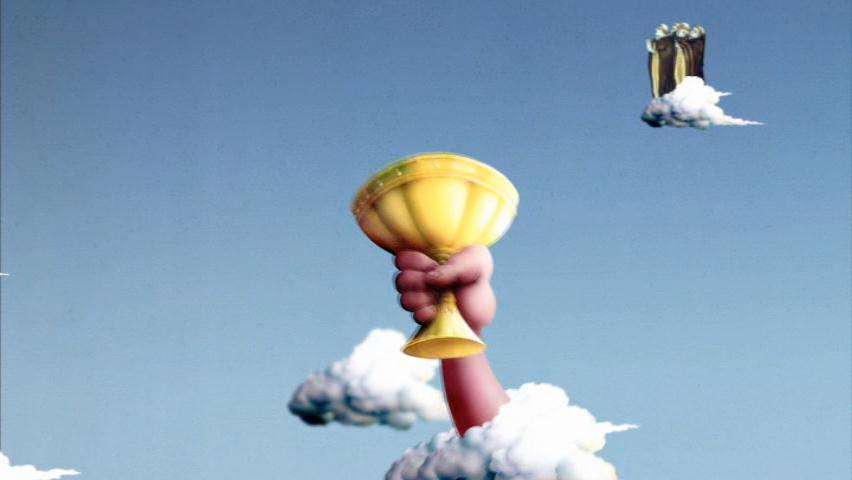
\includegraphics[width=0.8\textwidth]{grail.jpg}
%  \caption[Voorbeeld figuur.]{\label{fig:grail}Voorbeeld van invoegen van een figuur. Zorg altijd voor een uitgebreid bijschrift dat de figuur %volledig beschrijft zonder in de tekst te moeten gaan zoeken. Vergeet ook je bronvermelding niet!}
%\end{figure}

%\begin{listing}
%  \begin{minted}{python}
%    import pandas as pd
%    import seaborn as sns
%
%    penguins = sns.load_dataset('penguins')
%    sns.relplot(data=penguins, x="flipper_length_mm", y="bill_length_mm", hue="species")
%  \end{minted}
%  \caption[Voorbeeld codefragment]{Voorbeeld van het invoegen van een codefragment.}
%\end{listing}

%\lipsum[7-20]

%\begin{table}
%  \centering
%  \begin{tabular}{lcr}
%    \toprule
%    \textbf{Kolom 1} & \textbf{Kolom 2} & \textbf{Kolom 3} \\
%    $\alpha$         & $\beta$          & $\gamma$         \\
%    \midrule
%    A                & 10.230           & a                \\
%    B                & 45.678           & b                \\
%    C                & 99.987           & c                \\
%    \bottomrule
%  \end{tabular}
%  \caption[Voorbeeld tabel]{\label{tab:example}Voorbeeld van een tabel.}
%\end{table}

